
\chapter{Econophysics, Equilibrium, and Pareto}

This final chapter applies the Fokker--Planck formalism to a problem outside the financial markets: the \emph{distribution of wealth} in a population.
It is, in a sense, the purest piece of econophysics in the book --- no contracts, no hedging, just a statistical-mechanics question asked of society: if incomes diffuse randomly under simple rules, what stationary distribution do they reach?
The answer turns out to reproduce, from one and the same equation, the two regimes observed in every real economy: an exponential (Boltzmann) distribution for the lower and middle class, and a power-law (Pareto) tail for the rich.
% CLAUDE NOTE (unreviewed): These are the last two pages of PDF 6, unreviewed but
% clear in intent. Expansions and footnotes have been added for completeness.


\section{Power laws in economics}

Many phenomena, in economics and beyond, follow a \emph{power law}.
The classic example is \emph{Zipf's law}: rank the words of a text by frequency, and the frequency falls off as a power of the rank.
The same pattern appears in the sizes of cities, the sizes of firms, and --- the case that concerns us --- the distribution of wealth.

Wealth itself is hard to observe, so in practice one uses the \emph{gross income} $r$ (reddito) as a proxy, and studies the complementary CDF --- the fraction of individuals with income at least $r$ --- rescaled by the mean income $r/\bar r$ to compare across countries and years.
When this is done, the data speak clearly: two groups emerge.
The bulk of the population --- the lower and middle class --- follows an \emph{exponential} law; the wealthiest few percent follow a \emph{power-law} (Pareto) tail.
Figure~\ref{fig:wealth-dist} shows the two regimes in the form in which they appear in the empirical literature: in a log-linear plot the exponential bulk is a straight line from which the tail lifts off; in a log-log plot the Pareto tail is a straight line into which the bulk bends.
The power-law tail was discovered by Pareto in 1897\cite{Pareto1897}; the two-regime structure has been confirmed on modern data by Fujiwara, Champernowne, Yakovenko, and many others\cite{Yakovenko2009}, and its remarkable stability across countries and decades cries out for a mechanism.

% Figure replacing the multi-panel plot pasted in the raw notes (page 7);
% generated by images/code_for_images/wealth_distribution.py with parameters
% from Yakovenko & Rosser, Rev. Mod. Phys. 81, 1703 (2009).
\begin{figure}[h!]
\centering
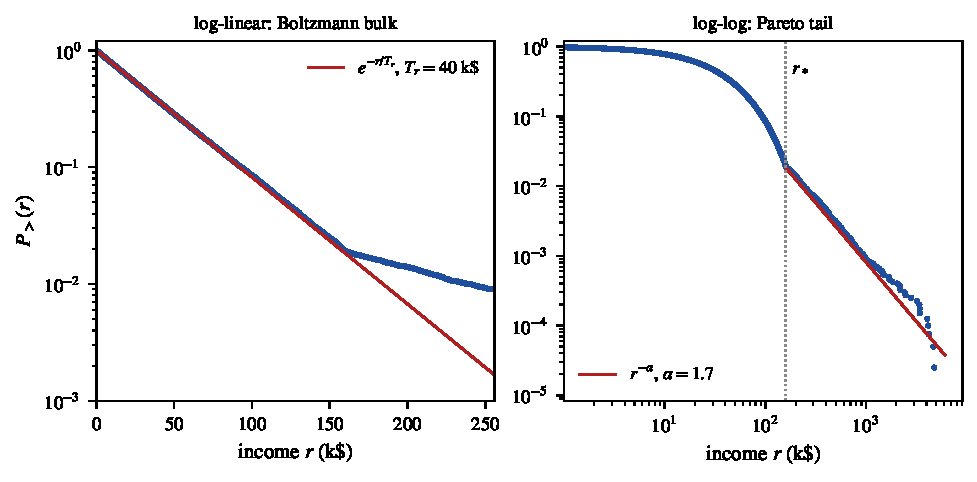
\includegraphics[width=0.95\textwidth]{images/wealth_distribution.pdf}
\caption{The two-regime income distribution, reproduced with the parameters reported for US data by Yakovenko \& Rosser\cite{Yakovenko2009}: an exponential (Boltzmann) bulk with income temperature $T_r\approx\$40$k covering $\sim97\%$ of the population, and a Pareto tail with exponent $\alpha=1.7$ above the crossover $r_*\approx4T_r$. Left, log-linear scale: the bulk is a straight line. Right, log-log scale: the tail is a straight line. Generated by \texttt{images/code\_for\_images/wealth\_distribution.py}.}
\label{fig:wealth-dist}
\end{figure}


\section{A diffusion model for income}\label{sec:income-diffusion}

The mechanism we propose is diffusion: incomes perform a stochastic process in ``income space''.
The physical distinction that will generate the two regimes is the \emph{source} of the income.
For the lower and middle class, income comes from labour --- wages, roughly deterministic, with additive fluctuations.
For the upper class, income comes from \emph{assets} --- capital gains, intrinsically stochastic, with fluctuations proportional to the capital itself.
One model, two regimes of its coefficients.

\subsection{General hypotheses}

The framework rests on four hypotheses.
\begin{enumerate}
    \item Incomes are divisible into an infinitely numerable set of income classes $r \in R_+$, with $r \ge r_{\min}$.
    \item $P(r,t)$ is the fraction of individuals with income $r$ at time $t$, and $N$ is the total number of income earners, so that $N\, P(r,t)\, dr = dm(r,t)\, dr$ counts the earners in $[r,r+dr]$.
    We take $N$ constant, since there is approximately a one-to-one map between individuals and income positions (people change salary, change job, inherit --- but the slots remain).
    \item The distribution is normalized, $\int P(r',t)\, dr' = 1$.
    \item The diffusion has \emph{no memory}: the process is Markov.
\end{enumerate}

\subsection{The master equation}

By hypothesis 4 and the results of Chapter~3, the master equation for $P(r,t)$ is a Fokker--Planck equation, with drift and diffusion coefficients $A(r)$ and $B(r)$:
\begin{equation}\label{eq:fp-income}
\frac{\partial}{\partial t}\, P(r,t) = \frac{\partial}{\partial r}\bigl[A(r)\, P(r,t)\bigr] + \frac{\partial^2}{\partial r^2}\bigl[B(r)\, P(r,t)\bigr],
\end{equation}
written here with the sign convention of the notes, in which
\begin{equation}
\frac{d}{dt}\langle r(t)\rangle = -\langle A(r)\rangle, \qquad \frac{d}{dt}\langle r^2(t)\rangle = \langle 2\,B(r)\rangle:
\end{equation}
a positive $A$ describes an average \emph{loss} of income, and $B$ the intensity of its fluctuations.

\subsection{Equilibrium (stationary) solution}

Now the economic input: empirically, the \emph{shape} of the income distribution is approximately constant over time --- individuals move up and down, but the histogram barely changes from year to year.
This is an equilibrium statement, and we implement it by the \emph{stationary} Fokker--Planck equation,
\begin{equation}
\frac{\partial}{\partial t}\, P(r,t) = 0.
\end{equation}
The right-hand side of~\eqref{eq:fp-income} then collapses into a total derivative,
\begin{equation}
0 = \frac{d}{dr}\bigl[A(r)\, P(r)\bigr] + \frac{d^2}{dr^2}\bigl[B(r)\, P(r)\bigr] = \frac{d}{dr}\biggl\{A(r)\, P(r) + \frac{d}{dr}\bigl[B(r)\, P(r)\bigr]\biggr\},
\end{equation}
and the object in braces is precisely the probability flux $J(r)$ of Chapter~3,
\begin{equation}
J(r) = A(r)\, P(r) + \frac{d}{dr}\bigl[B(r)\, P(r)\bigr],
\end{equation}
constant in $r$ by the equation above.
Requiring $P(r)\to 0$ both as $r\to 0$ and as $r\to\infty$ forces the constant to vanish, so $J=0$ everywhere:
\begin{equation}\label{eq:flux-zero}
A(r)\, P(r) + \frac{d}{dr}\bigl[B(r)\, P(r)\bigr] = 0.
\end{equation}
Equilibrium with zero flux --- detailed balance, a statistical mechanician would say (Appendix~\ref{app:stationary}) --- is a first-order ODE for $P(r)$: given any choice of $A$ and $B$, the stationary distribution follows by one integration.
It remains to feed in the economics.


\section{Lower and middle class}\label{sec:lower-class}

For the lower and middle class both coefficients are constants,
\begin{equation}
A(r) = A_0, \qquad B(r) = B_0 > 0.
\end{equation}
The reading is concrete.
A constant, positive $A_0$ describes a steady linear erosion of purchasing power, $\frac{d}{dt}\langle r(t)\rangle = -A_0$ --- wages nibbled by inflation, taxes, and living costs --- while the fluctuations have constant intensity, $\frac{d}{dt}\langle r^2(t)\rangle = 2B_0$: raises, job changes, small windfalls, all of a size that does not depend on how rich one already is.
This additivity is the statistical signature of \emph{labour} income.

With constant coefficients the stationary equation~\eqref{eq:flux-zero} becomes
\begin{equation}
A_0\, P(r) + B_0\,\frac{dP}{dr} = 0 \quad\Longrightarrow\quad \frac{dP}{P} = -\frac{A_0}{B_0}\, dr,
\end{equation}
and integrating,
\begin{equation}
\int\!\frac{dP(r')}{P(r')} = -\frac{A_0}{B_0}\,r' \quad\Longrightarrow\quad P(r) \propto C\, e^{-\frac{A_0}{B_0}\, r} = C\, e^{-r/T_r},
\end{equation}
an \emph{exponential} distribution (positive and normalizable provided $A_0 > 0$), with scale
\begin{equation}\label{eq:boltzmann-income}
T_r = \frac{B_0}{A_0}.
\end{equation}
The form is unmistakable to a physicist: it is a Boltzmann distribution (Appendix~\ref{app:ensembles}), $e^{-E/k_BT}$ with income in place of energy, and $T_r$ plays the role of an \emph{effective temperature of income} --- large when fluctuations ($B_0$) are strong relative to erosion ($A_0$); the general mechanism by which a zero-flux state of a diffusion acquires the Boltzmann form is spelled out in Appendix~\ref{app:stationary}.
At equilibrium the distribution is stable even though every individual income keeps fluctuating; and if the mean income $\langle r\rangle$ falls, the ``temperature'' falls with it, compressing the whole distribution.
Money, in this class, behaves like energy in a gas: exchanged in roughly equal quanta, conserved overall, and exponentially distributed at equilibrium.


\section{Upper class}\label{sec:upper-class}

For the upper class the phenomenology is different in kind, not just in degree: income is driven by \emph{multiplicative feedback}, because capital generates returns proportional to itself.
The coefficients that encode this are
\begin{equation}
A(r) = a\,r, \qquad B(r) = b\,r^2 \qquad (a, b > 0),
\end{equation}
giving
\begin{equation}
\frac{d}{dt}\langle r(t)\rangle = -a\,\langle r(t)\rangle,
\qquad
\frac{d}{dt}\langle r^2(t)\rangle = b\,\langle r^2(t)\rangle:
\end{equation}
the average relative erosion is the same as before, but the fluctuations now \emph{grow with the square of the income} --- positive feedback, the rich man's gains and losses both scaling with his fortune.
This multiplicativity is the statistical signature of \emph{asset} income, and the reader will recognize in $A\propto r$, $B\propto r^2$ the drift-diffusion structure of the geometric Brownian motion of Chapter~4.

We solve the stationary equation~\eqref{eq:flux-zero} with these coefficients.
Expanding the derivative,
\begin{equation}
A(r)\, P(r) + B(r)\,\frac{dP}{dr} + P(r)\,\frac{dB}{dr} = 0
\quad\Longrightarrow\quad
P'(r) + \frac{A(r) + B'(r)}{B(r)}\, P(r) = 0,
\end{equation}
and substituting $A(r) = ar$, $B(r) = br^2$, $B'(r) = 2br$,
\begin{equation}
P'(r) + \frac{ar + 2br}{br^2}\, P(r) = 0 \quad\Longrightarrow\quad P'(r) + \frac{a+2b}{b}\,\frac{1}{r}\, P(r) = 0.
\end{equation}
This is again a separable first-order ODE,
\begin{equation}
\frac{dP}{P} = -\frac{a+2b}{b}\,\frac{dr}{r},
\end{equation}
whose integral is worth organizing as in the notes: splitting the coefficient as $\frac{a+2b}{b} = \frac{a}{b} + 2$,
\begin{equation}
\int\!\frac{dP(r')}{P(r')} = -\int\!\frac{B'(r')}{B(r')}\, dr' - \int\!\frac{A(r')}{B(r')}\, dr',
\end{equation}
the first integral gives $\ln B(r) = \ln(br^2)$, and the second
\begin{equation}
\int\!\frac{A(r')}{B(r')}\, dr' = \frac{a}{b}\int\!\frac{dr'}{r'} = \frac{a}{b}\,\ln r,
\end{equation}
so that, for $r \gg r_0$,
\begin{equation}
P(r) \approx \frac{C}{B(r)}\, e^{-\int \frac{A(r')}{B(r')}\, dr'} = \frac{C}{b\,r^2}\, r^{-a/b},
\end{equation}
that is,
\begin{equation}\label{eq:pareto}
P(r) = C\, r^{-(2 + a/b)} = C\, r^{-(\alpha+1)},
\end{equation}
a \emph{power law}: the multiplicative structure has converted the exponential into a Pareto tail.
% CLAUDE NOTE: the notes write P(r) = C r^{-2} r^{-a/b} = C r^{-(1+a/b)-1} = C r^{-(1+α)},
% consistent with a CDF exponent α = 1 + a/b as stated below.
Correspondingly, the complementary CDF decays as $r^{-\alpha}$, with
\begin{equation}\label{eq:pareto-exponent}
\alpha = 1 + \frac{a}{b},
\end{equation}
the \textbf{Pareto exponent}.
Since $a, b > 0$, the model predicts $\alpha > 1$ automatically.
Empirically, fits across countries give $\alpha \approx 1.6$--$1.8$, which through~\eqref{eq:pareto-exponent} implies $b > a$: for the upper class, the multiplicative fluctuations of capital \emph{dominate} its average erosion --- and it is precisely this dominance of noise that populates the far tail of great fortunes.\footnote{A Pareto exponent $\alpha < 2$ means that the \emph{variance} of the income distribution diverges: inequality in the tail is so extreme that no ``typical spread'' exists. That $\alpha$ falls in the same narrow window for very different countries suggests that the mechanism --- multiplicative dynamics of capital --- is universal, largely indifferent to institutional detail.}

\medskip

It is worth stepping back to admire the unity of the result.
One Fokker--Planck equation, one zero-flux equilibrium condition; additive coefficients give Boltzmann's exponential for the many, multiplicative coefficients give Pareto's power law for the few, and the crossover between the two regimes is visible in the income data of every country.
The tools were exactly those of the rest of the book --- the same stationary Fokker--Planck equation that priced no options and hedged no portfolios here draws, with two lines of algebra, the statistical portrait of a society.
This is econophysics at its best: not finance dressed up in physics notation, but the genuine transfer of a physical way of thinking --- equilibrium, diffusion, universality --- to economic matter.


\section[The minority game*]{The minority game\texorpdfstring{$^*$}{*}}
% ============================================================================
% BLANK SECTION (placeholder, added at the author's request on 2026-07-06).
% Planned content: the Minority Game of Challet & Zhang (1997) as the agent-based
% counterpart of this chapter — N adaptive agents, public information α = P/N,
% the volatility curve σ²/N, the phase transition at α_c ≈ 0.337, and its exact
% solution by the replica method (Challet, Marsili & Zecchina 2000).
% The asterisk marks material beyond the handwritten notes and the course program.
% ============================================================================

\begin{center}
\fbox{\parbox{0.85\textwidth}{%
\textbf{Note:} This section is a placeholder, to be written.
It will present the \emph{minority game} --- the simplest agent-based model of a market of adaptive, heterogeneous, competing agents --- and its phase transition between an efficient and an inefficient phase, solved exactly with the statistical mechanics of disordered systems.
}}
\end{center}
